% COMMANDS
\newcommand{\reporttitle}{Himeno benchmark}
\newcommand{\hb}{\textit{Himeno Benchmark}}
\newcommand{\jm}{\textit{Jacobi method}}

\documentclass[english, 11pt]{tudscrartcl}
\iftutex
    \usepackage{fontspec}
\else
    \usepackage[T1]{fontenc}
\fi

% OPTIONS
\KOMAoptions{
    titlepage=true
}

\usepackage{babel}

% For math
\usepackage{amsfonts}
\usepackage{amsmath}
\usepackage{interval}
\newcommand{\floor}[1]{\left\lfloor #1 \right\rfloor}

% For tables
\usepackage{tabularx}
\usepackage{makecell}
\usepackage{multirow}
\usepackage{booktabs}

% For listings (code blocks)
\usepackage{listings}
\lstset
{ %Formatting for code in appendix
    basicstyle=\footnotesize\ttfamily,
    numbers=left,
    stepnumber=1,
    showstringspaces=false,
    tabsize=4,
    breaklines=true,
    breakatwhitespace=false,
}

% For references
\usepackage{nameref}
\usepackage{hyperref}

% For figures
\usepackage{graphicx}
\usepackage{rotating}
\usepackage{lscape}
\usepackage{calc}

% Spacings
\usepackage{enumitem}\setlist{noitemsep}
\newcommand{\setspacings}{
    \baselineskip=15pt
    \parskip=10pt
    \parindent=0pt
}

% TITLE
\faculty{Computer Science}
\institute{Institute of Systems Architecture}
\chair{Chair of Systems Engineering}
\date{\today}

\author{%
    Fritz Louis Wilke%
    \emailaddress*{E-Mail: fritz.wilke@tu-dresden.de}%
    \matriculationnumber{4536116}%
    \discipline{M. Sc. Computer Science}%
    \course{INF-MA-PR (graded)}%
}


\title{\reporttitle}
\subtitle{Lab: Concurrent and Distributed Systems}
\begin{document}

\setspacings
\maketitle

% The report content starts here
\clearpage
\setcounter{page}{1}

% INTRODUCTION
\section{Introduction}
\label{sec:introduction}

This report is part of the \textit{Concurrent and Distributed Systems Lab} which aims to test and improve practical knowledge about scalable, parallel programming.

\subsection{The Problem}
\label{ssec:problem}

The \hb{} is - as the name implies - a benchmarking program. It was developed by Dr. Ryutaro Himeno at the RIKEN Institute in 1996, but the \href{https://i.riken.jp/en/supercom/documents/himenobmt/}{source code} is still available today. Its goal is to provide a comparable, overall performance benchmark between different machines and architectures. This includes the memory throughput, caching behaviour and CPU performance (FLOPS).

The program requires four inputs. The $rows$, $cols$ and $deps$ define three of four sizes of the 4D-matrices to work with and $nn$ is used to specify the number of \textit{Jacobi} iterations performed. The \jm{} is an iterative algorithm to determine the solutions of a system of linear equations. Usually, the \jm{} is executed until the solution converges, but in this program the number of iterations is defined by $nn$.

The output of the program is calculated in the last iteration of the \jm{} and is called the \textit{Gosa number}. In a nutshell, the \textit{Gosa number} is the sum of the squared average of the direct neighbours of each voxel $v_{ijk} \in M$, where $M$ is the current three dimensional working matrix.

The task of this lab is to find a way to parallelize the described program in a way that it scales well with an increasing number of available CPUs. To achieve this, strategies of concurrent and distributed systems programming are used to plan, implement and evaluate the parallelized program. The provided output must match the one given by the sequential solution, though the algorithm itself may be modified. Note that it is not the goal of the parallelized program to provide a comparable benchmark, as it is intended by the original program.


\subsection{Unoptimized Code Base}
\label{ssec:code-base}

\begin{lstlisting}[caption={Simplified Pseudo Code of the unoptimized Algorithm}, label={lst:pseudo-code-original}, captionpos=b, frame=tb, float]
input: uint rows, uint cols, uint deps, uint nn
output: float
begin
    // creates and initializes the global 4D matrices: a, b, c, p, bnd, wrk1, wrk2
    initialize_matrices()
    
    let gosa = 0.0
    for n in 0..nn:
        gosa = 0.0
    
        // iterate over every voxel (at layer 0)
        for r in 1..rows-1:
            for c in 1..cols-1:
                for d in 1..deps-1:
                    let ss = jacobi_iteration(r, c, d) // can be seen as a blackbox for now
                    gosa += ss*ss
                    wrk2[0][r][c][d] = p[0][r][c][d] + 0.8*ss
                    
        wrk2.copy_to(p) // copy content of p to wrk2
    
    print( gosa ) // print result (with a precision of 6)
end
\end{lstlisting}

Ryutaro Himeno's source code is written in C. This code forms the basis for the development of the program. Its basic workflow is summarized as pseudo code in Listing \ref{lst:pseudo-code-original}. As already mentioned in the \hyperref[sec:introduction]{introduction}, the benchmark works with 4D matrices which are initialized with defined values. Note that the three dimensional size of the matrices is identical, they only differ in the fourth (outermost) dimension.

For each iteration \verb+n+, the \verb+gosa+ gets set to zero. After that, the program iterates over every \textit{voxel} to execute its calculations on it. A \textit{voxel} is like a pixel with three dimensions, as it defines a position in a three dimensional matrix. In the next step, the gosa gets increased with the squared result \verb+ss+ that was previously calculated. Finally, the \verb+wrk2+ matrix is set at the current voxel, with the content of the matrix \verb+p+ plus 0.8th of \verb+ss+.

The last step in the iteration \verb+n+ is to copy the content of the matrix \verb+wrk2+ to the matrix \verb+p+. These contents are then used in the next iteration. Finally, when \verb+nn+ iterations have been executed, the \textit{Gosa number} is printed. In this task, the precision used for printing it is six. Seeing the applied loops, this algorithm has the complexity $\mathcal{O}(nn*2*(r-2)*(c-2)*(d-2))$, where the variables are the \textit{iteration amount} and \textit{rows}, \textit{cols} and \textit{deps} of the matrices in that order. The computational expense used for the initialization of the matrices is not included in that estimate. The $2*$ comes from the copy operation, since it is implemented by iterating element-wise over the source matrix.


\section{Optimization Strategies}
\label{sec:strategies}

To improve the scalability of the shown algorithm, several strategies have been developed and tested. The hard part of developing scalable software (w.r.t. the amount of CPU cores) is to distribute the given workload equally between the CPU cores while still having a correct result in the end. The two most successful strategies are presented in the following sections.

\subsection{Strategy I: Equal Work Distribution}
\label{ssec:strategy-i}

The goal of this strategy is to find a way to split the workload equally, \textbf{before} the actual computation starts. As the amount of calculations only depends on the given parameters and does not vary at runtime, the workload can be seen as fixed. Accordingly, it is a reasonable approach to simply split the workload into equal parts, one for each \textit{worker thread}. It is expected that each calculation takes the same amount of CPU cycles, or else this concept will not succeed. If one \textit{worker thread} finishes earlier than another, then it will go idle and it wastes parallel computation power.

Finding such a way to split workload is not trivial, especially having only the source code by hand. The simplified pseudo code in listing \ref{lst:pseudo-code-original} makes this already a bit easier. Usually, it is the best solution to parallelize the \textit{outermost} loop. Unfortunately, the iterations from zero to $nn$ (line 8) depend on each other and can thus not be parallelized directly. It can be seen that the matrix $wrk2$ depends on $p$ (line 17), whereas $p$ depends on $wrk2$ (line 19) in the same iteration $n$ later on. Thus, $p$ ultimately depends on itself of the previous iteration $n-1$. Having said this, the next loop in the hierarchy would be a feasible target, which is the $rows$ loop in line 12. There is no dependence of rows \textbf{inside} an iteration $n$. If the amount of concurrent threads of the runtime environment is $t$, then each \textit{worker thread} receives $\omega = (rows-2) / t$ rows to calculate the new \verb$wrk2[0][r][c][d]$ values of. The threads get created and are joined for each iteration $n$, thus creating $nn*t$ threads throughout the runtime of the program. Since the creation of threads takes only a few microseconds it should not hurt the performance too much, respecting that $rows*cols*deps$ is much greater than $nn$.

This strategy should improve the performance due to the following reasons:
\begin{itemize}
    \item No synchronization overhead, only some overhead due to thread creation and joining
    \item No threads needed to distribute workload which causes inter-thread or even inter-socket communication
    \item Parallelizing the most work intensive calculations, namely the lines 15-17 of listing \ref{lst:pseudo-code-original}
\end{itemize}

One should keep in mind that there will still be a lot cache invalidation since the \hb{} is extremely memory intensive. This can be seen in the source code to which line 15 in listing \ref{lst:pseudo-code-original} relates. These widely distributed matrix accesses will almost always result in a cache miss, since only voxel neighbours on the \textit{deps} axis reside in continuous memory. It is not possible to prevent this behaviour.


\subsection{Strategy II: Atomic Variable}
\label{ssec:strategy-ii}

This strategy uses a shared atomic variable $v_{shared}$ to distribute the workload. The shared variable contains the next work portion for a \textit{worker thread} and can be accessed and modified in a \textbf{thread safe} manner. The \textit{worker thread} then calculates its assigned work and gets more once it is done. An atomic variable can be seen as a shared variable with a mutex that is used to prevent simultaneous variable access from multiple threads.
This strategy does not necessarily expect that each \textit{worker thread} calculates as fast as the others. It can thus cope with unforeseen scheduling behaviour that results in threads being delayed. The balancing act is to find a loop that is fine enough (inner loops) to make equal distribution possible but also coarse enough (outer loops) to prevent frequent, concurrent access of the shared variable. Since memory access is comparably slow to cache access, it should be avoided to access a shared variable too often.

Having said this, the \textit{rows} or \textit{cols} loop (line 12 and 13 in listing \ref{lst:pseudo-code-original}) are justified candidates for the shared variable. If the \textit{rows} loop is used, the content of the shared variable is trivial: simply put the next, not yet calculated row in it and increase by one when reading it. When working more fine grained and using the \textit{cols} loop, things get more tricky since the variable must also contain the information of the current \textit{row}. A simple solution would be to not only store the current col of the current row ($v_{shared} \in \interval{1}{rows-1}$) which would need two shared variables, but also \textbf{contain} the current row \textbf{implicitly} ($v_{shared} \in \interval{0}{(rows-2)*(cols-2)}$). The current row and col would be derived like this:
\begin{align*}
    row &= 1 + \floor{v_{shared} \div (cols-2)} \\
    col &= 1 + v_{shared} \bmod (cols-2)
\end{align*}

This strategy should improve the performance due to the following reasons:
\begin{itemize}
    \item Parallelizing the most work intensive calculations, namely the lines 15-17 of listing \ref{lst:pseudo-code-original}
    \item The ability to cope with unforeseen delays of threads (eg. due to scheduling)
    \item Not having too frequent accesses on the shared variable $v_{shared}$
\end{itemize}

It can be seen that this strategy provides advantages similar to strategy I. However, this strategy can cope with different CPU times of the \textit{worker threads}, whereas strategy I cannot. If the CPU time gets distributed evenly throughout the threads though, using and accessing a shared variable would be an unnecessary slow down.


\section{Implementation}
\label{sec:implementation}

This section presents the most important implementation details of the optimized program. At first, general improvements on the code are elaborated, which also affect the single thread performance. The latter subsection focuses on the improvements that have been made specifically for multithreading.

\subsection{General Improvements}
\label{ssec:general-improvements}

Having a closer look into Himeno's source code, one may observe that there are a lot memory accesses which are also widely scattered w.r.t. locality. This is a killer for multithreaded performance since it makes the usage of CPU caches almost forfeited. As long as \textit{cache thrashing} occurs, it is hard to parallelize the program efficiently because the speed of memory accesses is the limiting factor. An important objective would therefore be to \textbf{reduce memory usage} as far as possible.

Inspecting the matrix accesses, it can be seen that the matrices $a$, $b$, $c$, $bnd$ and $wrk1$ are never modified. Theses matrices can be replaced by constants which reduces the memory usage drastically. The constants for the matrices at are:
\begin{align*}
    a[0..2] &:= 1; a[3] := 1/6 \\
    b &:= 0 \\
    c &:= 1 \\
    bnd &:= 1 \\
    wrk1 &:= 0
\end{align*}

Multiplications with these constants can be optimized further on by \textbf{removing} products of zero multiplications (matrix $b$ and $c$) and simplifying multiplications with one (matrix $a[0..2]$, $c$ and $bnd$). The only matrices that are still in use after these modifications are matrix $a$ at layer 3 ($a[3] := 1/6$) as constant and the mutable matrices $p$ and $wrk2$.

Another, more obvious optimization target is the copy operation from line 19 of listing \ref{lst:pseudo-code-original}. This can be replaced with a simple variable swap. If $wrk2$ and $p$ are both \textbf{pointers} to matrices, then the following code reduces the complexity of the copy operation from $\mathcal{O}((r-2)*(c-2)*(d-2))$ (exponential) to $\mathcal{O}(1)$ (constant): \verb+std::swap(p, wrk2)+.

Furthermore, the matrix sizes can be reduced. An inspection of the code reveals that the outermost \textit{rows}, \textit{cols} and \textit{deps} are read but \textbf{never written}. Therefore the matrices can be reduced by two in every dimension. To prevent reads that are out of bound, a new function is implemented that calculates these read-only values on-the-fly when accessing out of bounds. Else, the actual matrix values are returned.

The last big optimization is the calculation of the \textit{Gosa number}. Since it is set to zero at the beginning of each iteration $n$ (see line 9 in listing \ref{lst:pseudo-code-original}), it is sufficient to only calculate it in the last iteration. This saves the execution of line 16 in listing \ref{lst:pseudo-code-original} for every iteration, excluding the last. Note that for the sake of readability of the source code, it was ported from C to C++, so that an own class can be created for the matrices and other quality of life features are available.

\subsection{Parallel Implementation}
\label{ssec:parallel_implementation}

Despite the general improvements mentioned in the previous section, not much code had to be changed. We assume that \hyperref[ssec:strategy-ii]{strategy II} provides better scalability than the first one since one can always expect variable calculation times of the same work when using several concurrent threads, especially when they're not bound to specific CPUs. The calculation is parallelized on the \textit{rows} loop, namely line 12 in listing \ref{lst:pseudo-code-original}. This should reduce the simultaneous access on the shared variable enough to prevent unwanted side effects.

The workflow of the parallel program is summarized as follows:
\begin{enumerate}
    \item Read the parameters from \verb+stdin+
    \item Create and initialize the two matrices \verb+p+ and \verb+wrk+
    \item For each iteration $n \in \interval{1}{nn}$ do:
    \begin{enumerate}
        \item Create $t-1$ \textit{worker threads}, matching the hardware concurrency
        \item Let the threads (including the main thread) calculate until there is no work left. The work is received by \textit{reading and incrementing} the shared variable.
        \item If it is the last iteration: modify the \textit{Gosa} variable (in a thread safe way)
        \item Join the \textit{worker threads}
        \item Swap the pointers of the matrices \verb+p+ and \verb+wrk+
    \end{enumerate}
    \item Print the \textit{Gosa number} that was calculated in the last iteration
\end{enumerate}

For the given task it is possible to implement and evaluate two different versions: one using 32 bit floating point variables (single precision or \textit{F32}) and one using 64 bit floating point variables (double precision or \textit{F64}). Due to the lack of precision using \textit{F32} variables, it is not possible to use partial sums of the \textit{Gosa number} for each thread. Therefore, the \textit{Gosa} variable must be shared throughout the \textit{worker threads} when using \textit{F32} variables to prevent an invalid result. As a consequence, the \textit{Gosa} variable is protected by a mutex in the \textit{F32} version.

The \textit{F64} versions (implemented in C++ and Rust) are not tied to this restriction. Each individual \textit{worker thread} uses its own \textit{F64} variable to sum up the \textit{Gosa number} using the voxels it worked with. Once every thread terminates, the partial sums of the threads merge to a correct result. Therefore, no locking is needed to calculate the \textit{Gosa number} in the \textit{F64} versions.

Rust is chosen as an alternative programming language to test the performance of another modern, hardwarenear language and also to learn a new programming language. Rust provides similar programming paradigms as C++, allowing it to compare the measurement results to the other implementation. The unoptimized Rust program, which is used for the absolute speedup calculation, is developed as close as possible to the original C code from Himeno. Note that only the \textit{F64} version is implemented in Rust.

\section{Evaluation}
\label{sec:evaluation}

\begin{table}[bt]
    \centering
    \begin{tabularx}{\textwidth}{crlrrrcX}
        \toprule
        
        &
        &
        &
        &
        \multicolumn{2}{c}{\thead{\textbf{Speedup@56}}} &
        &
        \\
        
        \cmidrule{5-6}
        
        \thead{\textbf{Lang.}} &
        \thead{\textbf{FXX}} &
        \thead{\textbf{Measurement}} &
        \thead{\textbf{Time@56}\\\textbf{{[ms]}}} &
        \thead{\textbf{abs}} &
        \thead{\textbf{rel}} &
        \thead{\textbf{Git Hash}} &
        \thead{\textbf{Evaluation Log}} \\
        
        \midrule
        
        \multirow{4}{*}[-0.75em]{C++} &
        \multirow{2}{*}[-0.25em]{32} &
        Unmodified &
        171978 &
        1x &
        1x &
        \href{https://se-gitlab.inf.tu-dresden.de/FLWilke/cds-s-2021/-/blob/c4e204b77e805787b6aaa5fb318883e5395b5320/tasks/mopp-2018-t3-himeno/himeno_original.c}{\texttt{c4e204b7}} &
        \href{https://cds-lab.pages.se-gitlab.inf.tu-dresden.de/cds-s-2021/cds-website/logs/c75cb293de1ed36a6bb94494fd0b3b8f3b23c2290f5a165617ce8b8dc5681fe8/2021-04-30T20:17:30+02:00.html}{30.04.2021 20:17:30} \\
        
        \cmidrule{3-8}
        
        &
        &
        Parallel &
        34346 &
        5x &
        10x &
        \href{https://se-gitlab.inf.tu-dresden.de/FLWilke/cds-s-2021/-/blob/43c3df53ecea64e10961dca8c41823ed766cba4c/tasks/mopp-2018-t3-himeno/himeno.cpp}{\texttt{43c3df53}} &
        \href{https://cds-lab.pages.se-gitlab.inf.tu-dresden.de/cds-s-2021/cds-website/logs/c75cb293de1ed36a6bb94494fd0b3b8f3b23c2290f5a165617ce8b8dc5681fe8/2021-05-09T16:17:19+02:00.html}{09.05.2021 16:17:19} \\
        
        \cmidrule{2-8}
        
        &
        \multirow{2}{*}[-0.25em]{64} &
        Unmodified &
        207050 &
        1x &
        1x &
        \href{https://se-gitlab.inf.tu-dresden.de/FLWilke/cds-s-2021/-/blob/c4e204b77e805787b6aaa5fb318883e5395b5320/tasks/mopp-2018-t3-himeno/himeno_original.c}{\texttt{c4e204b7}} &
        \href{https://cds-lab.pages.se-gitlab.inf.tu-dresden.de/cds-s-2021/cds-website/logs/c75cb293de1ed36a6bb94494fd0b3b8f3b23c2290f5a165617ce8b8dc5681fe8/2021-04-30T20:17:30+02:00.html}{30.04.2021 20:17:30} \\
        
        \cmidrule{3-8}
        
        &
        &
        Parallel &
        19294 &
        10x &
        \textbf{17x} &
        \href{https://se-gitlab.inf.tu-dresden.de/FLWilke/cds-s-2021/-/blob/43c3df53ecea64e10961dca8c41823ed766cba4c/tasks/mopp-2018-t3-himeno/himeno.cpp}{\texttt{43c3df53}} &
        \href{https://cds-lab.pages.se-gitlab.inf.tu-dresden.de/cds-s-2021/cds-website/logs/c75cb293de1ed36a6bb94494fd0b3b8f3b23c2290f5a165617ce8b8dc5681fe8/2021-05-09T16:17:19+02:00.html}{09.05.2021 16:17:19} \\
        
        \midrule
        
        \multirow{2}{*}[-0.25em]{Rust} &
        \multirow{2}{*}[-0.25em]{64} &
        Unoptimized &
        289943 &
        1x &
        1x &
        \href{https://se-gitlab.inf.tu-dresden.de/FLWilke/cds-s-2021/-/blob/3773b864db7acb4119fcc3bcc1b6484da376feee/tasks/mopp-2018-t3-himeno-rust-unoptimized/src/main.rs}{\texttt{3773b864}} &
        \href{https://cds-lab.pages.se-gitlab.inf.tu-dresden.de/cds-s-2021/cds-website/logs/c75cb293de1ed36a6bb94494fd0b3b8f3b23c2290f5a165617ce8b8dc5681fe8/2021-05-12T16:17:25+02:00.html}{12.05.2021 16:17:25} \\
        
        \cmidrule{3-8}
        
        &
        &
        Parallel &
        \textbf{7108} &
        \textbf{43x} &
        16x &
        \href{https://se-gitlab.inf.tu-dresden.de/FLWilke/cds-s-2021/-/blob/3fadcfc33229b180e11c31f4d9eb98d393ce9a33/tasks/mopp-2018-t3-himeno-rust/src/main.rs}{\texttt{3fadcfc3}} &
        \href{https://cds-lab.pages.se-gitlab.inf.tu-dresden.de/cds-s-2021/cds-website/logs/c75cb293de1ed36a6bb94494fd0b3b8f3b23c2290f5a165617ce8b8dc5681fe8/2021-05-26T20:17:11+02:00.html}{26.05.2021 20:17:11} \\
        
        \bottomrule
    \end{tabularx}
    \caption{Evaluation Results of the Implementations}
    \label{tab:evaluation-results}
\end{table}

The previously described parallel implementations are evaluated in this chapter. All important measurement results can be seen in table \ref{tab:evaluation-results}, categorized by their programming language and the used floating point precision. The shown \textbf{absolute speedup} is the speedup of the evaluated program using 56 concurrent threads with respect to the runtime of the unoptimized program (using 56 concurrent threads). The \textbf{relative speedup} refers to the runtime of the same program and evaluation run using only a single thread. This speedup is also shown in detail in figure \ref{fig:scaling}. The evaluated source code and commit is available using the Git hash which includes a hyperlink to the source file.

It can be seen in table \ref{tab:evaluation-results} that the best overall runtime results from the multithreaded Rust implementation, which took around seven seconds. It is followed by the \textit{F64} C++ implementation with 19 seconds and \textit{F32} C++ program that ran 34 seconds. The \textbf{absolute speedups} are 43, 10 and five respectively. Remind that these speedups refer to the unoptimized programs. The best relative speedup is achieved by the \textit{F64} C++ implementation. This program reached a \textbf{relative speedup} of 17 using 56 concurrent threads.

The same code accomplished a relative speedup of ten using \textit{F32} variables. The lower speedup can be concluded from the shared \textit{Gosa} variable mentioned in the previous chapter. It seems that this is the limiting factor which prevents the program from scaling higher than ten. The graph in figure \ref{fig:scaling} (left) shows this limit very well. There is no significant performance increase from using 28 concurrent threads or more. This graph also shows a strong performance decrease when using 16 threads. This is because after 15 or more threads, the second CPU socket is used, forcing the hardware to communicate via the slow CPU BUS.

This performance collapse can also be discovered in the other two graphs in figure \ref{fig:scaling}. However, there is no sharp scaling limit on the \textit{F64} implementations. The C++ version even resembles the curve of \textit{Amdahl's law}. Using Amdahl's law, the parallel code amount for the C++ \textit{F64} implementation is 97.37\% at 28 threads and 95.92\% using 56 threads. The parallel code amount for the \textit{F32} is 93.46\% and 91.91\% for 28 and 56 threads respectively. The Rust version results in 96.44\% and 95.36\% parallel code. These results seem realistic, but due to the unstable scaling curve, a precise upper scaling limit can not be predicted using Amdahl's law. The \nameref{sec:appendix} contains graphs showing the curve of Amdahl's law with these parallel code parts.

\begin{figure}[bt]
    \hspace*{-\oddsidemargin}\makebox[\textwidth]{
        \centering
        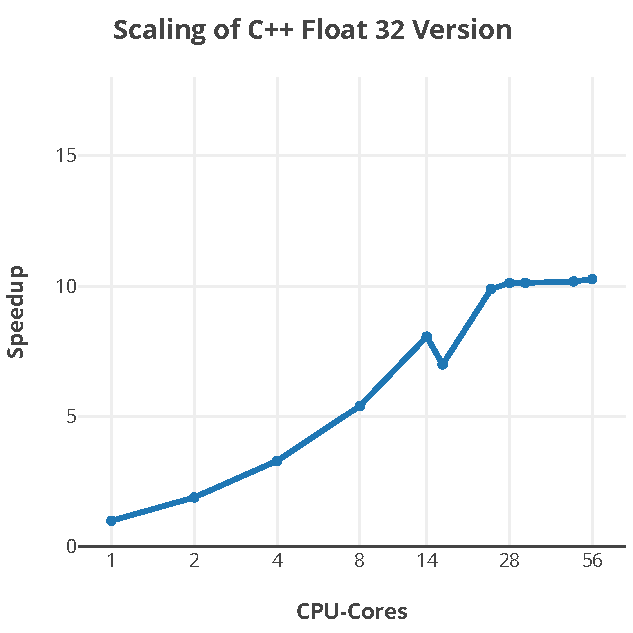
\includegraphics[width=0.32\paperwidth]{himeno/assets/himeno_4-scaling.pdf}
        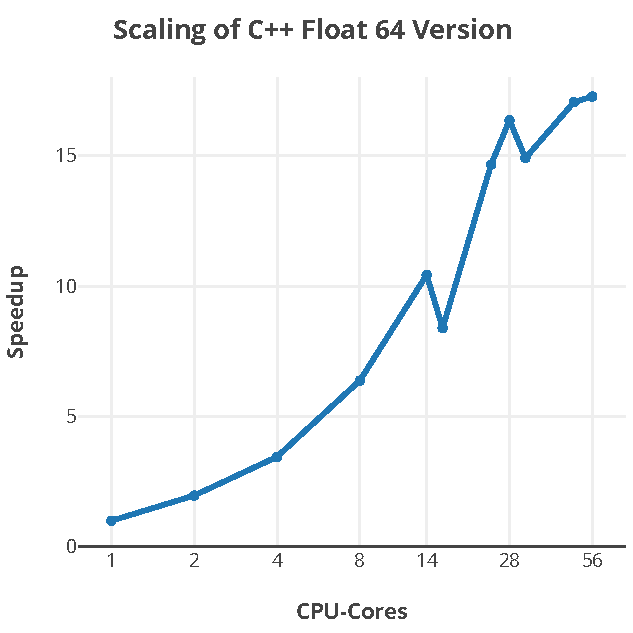
\includegraphics[width=0.32\paperwidth]{himeno/assets/himeno-float64_4-scaling.pdf}
        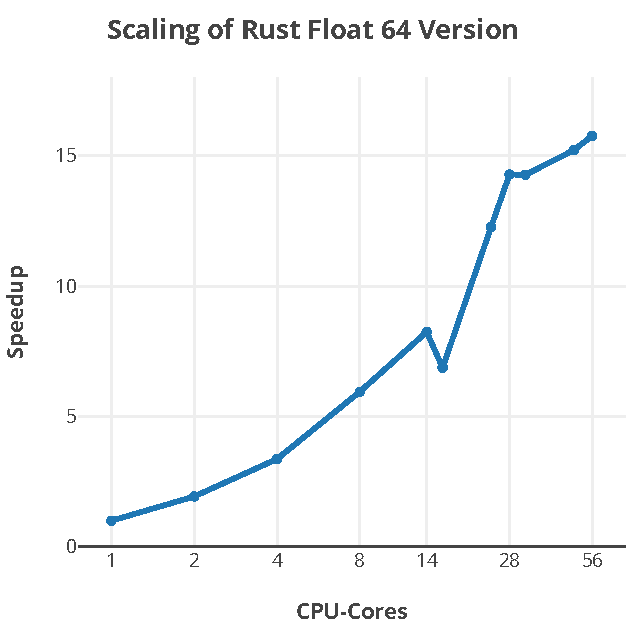
\includegraphics[width=0.32\paperwidth]{himeno/assets/himeno-rust_2-scaling.pdf}
    }
    \caption{Scaling of the C++ Versions Float 32 (left), Float 64 (middle) and Rust Float 64 (right)}
    \label{fig:scaling}
\end{figure}



\section{Conclusion}
\label{sec:conclusion}

The desired optimal speedup of 13 is surpassed by both, the \textit{F64} C++ and Rust implementation. Due to the memory intensive nature of the \textit{Himeno Benchmark}, the scaling behaviours of the programs are neither smooth nor spectacularly high, but they show a satisfying efficiency in comparison to the unoptimized programs. It is shown that it suffices to implement basic multithreading strategies in combination with general code optimizations to reach this speedup.


\clearpage
\thispagestyle{empty}

\newlength{\topmarginlength}
\setlength{\topmarginlength}{1in+\voffset+0.5\headsep+0.5\footskip}
\begin{landscape}
    \section{Appendix}
    \label{sec:appendix}

    \begin{figure}[h]
        \hspace*{\topmarginlength}\makebox[\textwidth]{
            \centering
            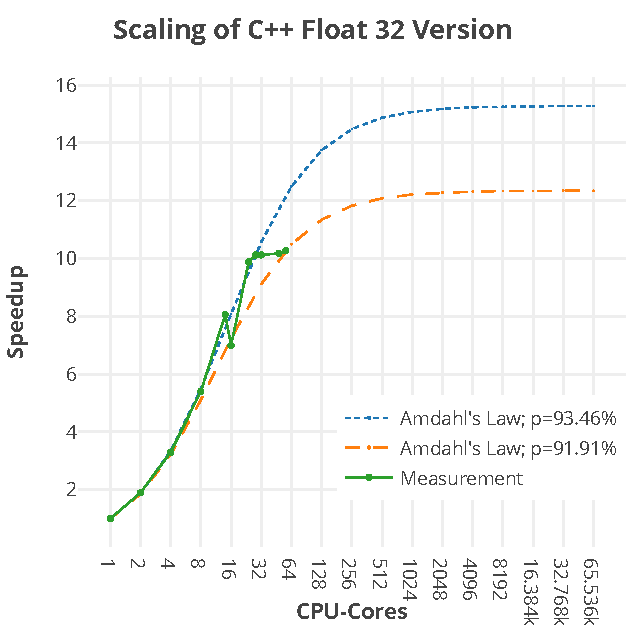
\includegraphics[width=0.32\paperheight]{himeno/assets/himeno_4-amdahls-law.pdf}
            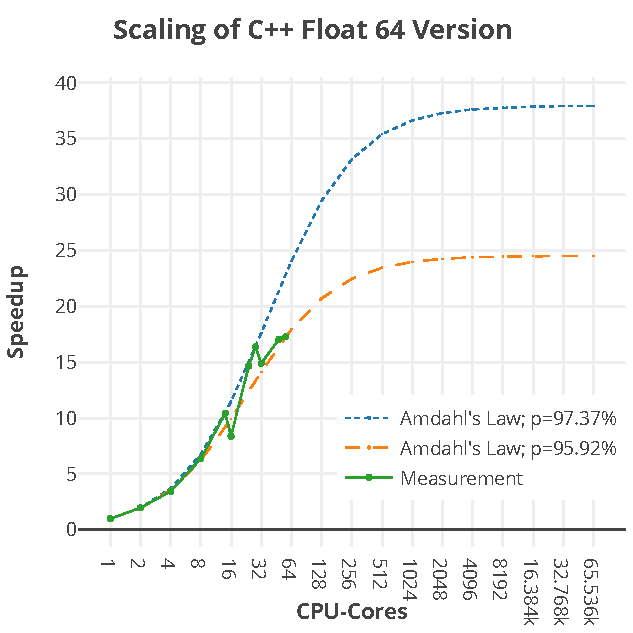
\includegraphics[width=0.32\paperheight]{himeno/assets/himeno-float64_4-amdahls-law.pdf}
            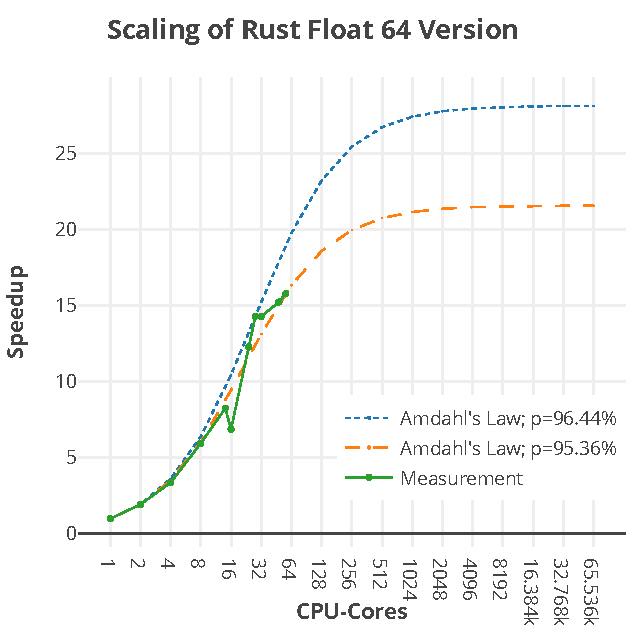
\includegraphics[width=0.32\paperheight]{himeno/assets/himeno-rust_2-amdahls-law.pdf}
        }
        \caption{Scaling of the C++ Versions Float 32 (left), Float 64 (middle) and Rust Float 64 (right) enhanced with Amdahl's law}
        \label{fig:scaling-amdahls-law}
    \end{figure}
\end{landscape}

\end{document}